\part{Il problema}

\begin{frame}
	\partpage
	\centering
\end{frame}

\begin{frame}
	\frametitle{Reti complesse}
	\centering
	\begin{figure}[h]
		\centering
		\begin{flushleft}
			Grafi con caratteristiche topologiche non banali che occorrono modellando 
			
			sistemi reali (quali social network, computer network, collaboration network...).
		\end{flushleft}
		\medskip
		
		\pause
		\small 
		\begin{minipage}[t]{.45\textwidth}
			\centering
			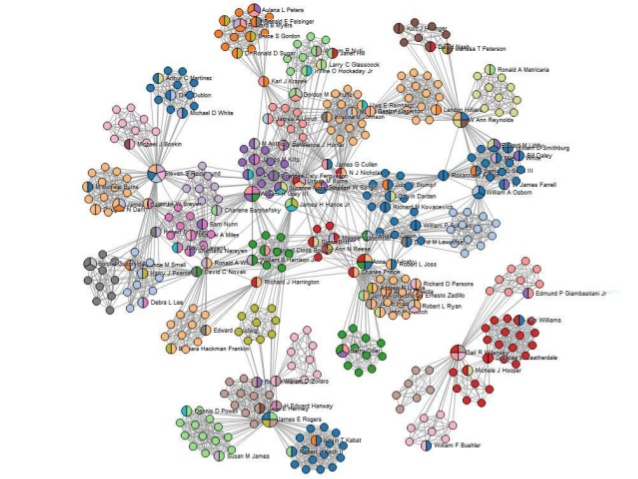
\includegraphics[width=1\textwidth]{images/9_social}
			\small 
			\caption{Cluster di amicizie in un social network } % \\ \textit{Fonte: SNAP Stanford}}
		\end{minipage}\hfill
		\pause
		\begin{minipage}[t]{.45\textwidth}
			\centering
			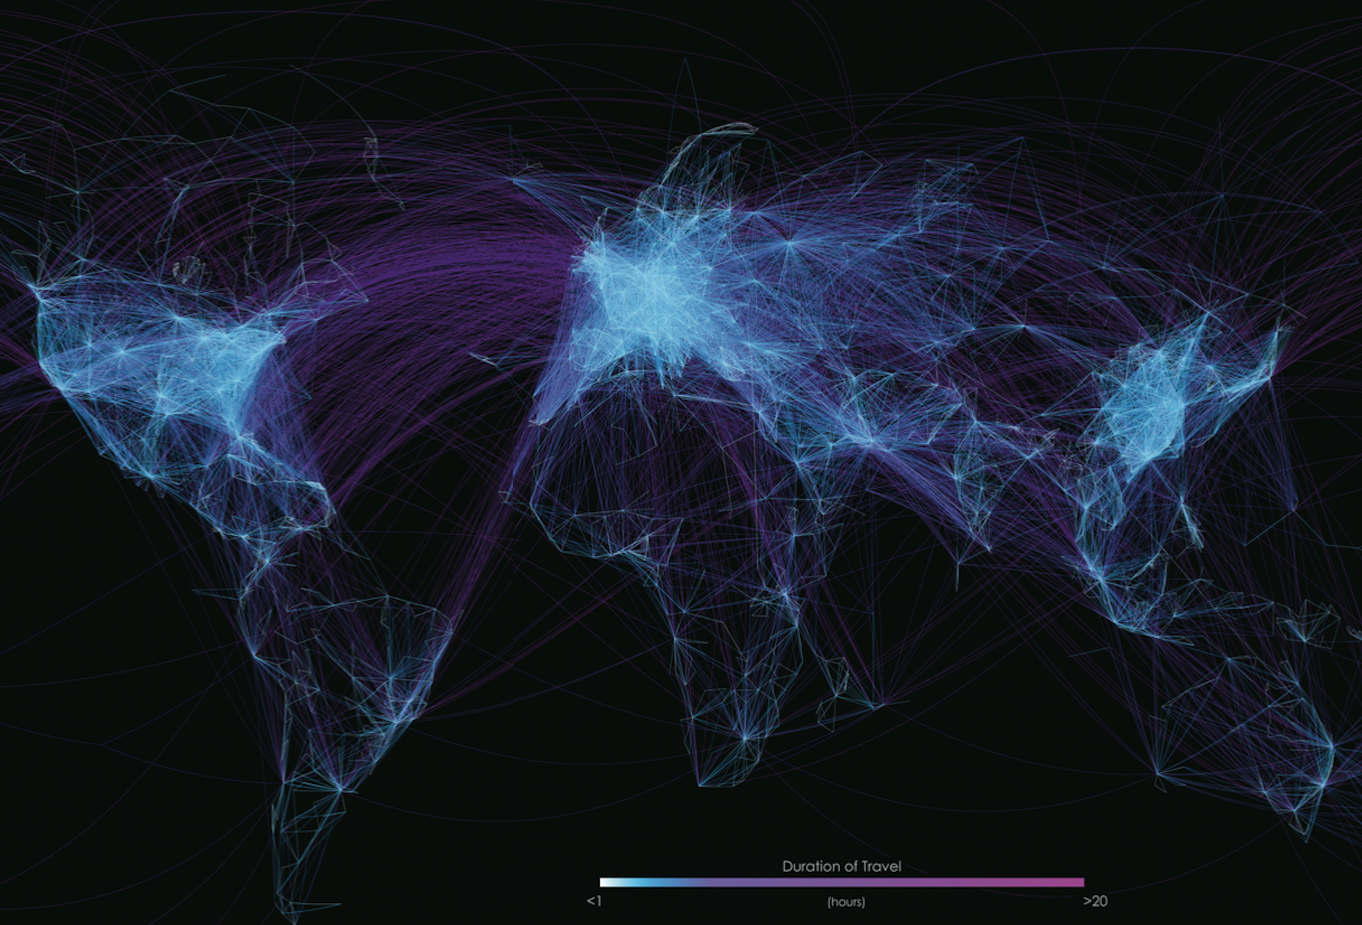
\includegraphics[width=1\textwidth]{images/7_flight}
			\small 
			\caption{Rotte dei voli commerciali} % \\ \textit{Fonte: Bio Diaspora, Toronto}}
		\end{minipage}
	\end{figure}
\end{frame}

\begin{frame}
	\frametitle{Indici di similarità}
	\centering
	
	\small
	\pause
	\begin{figure}[h]
		\begin{minipage}[t]{.48\textwidth}
			\centering
			\Large
			Jaccard
			\small
			\medskip
			\begin{equation*}
				J(A,B) = \frac{|A \cap B|}{|A \cup B|}
			\end{equation*}
			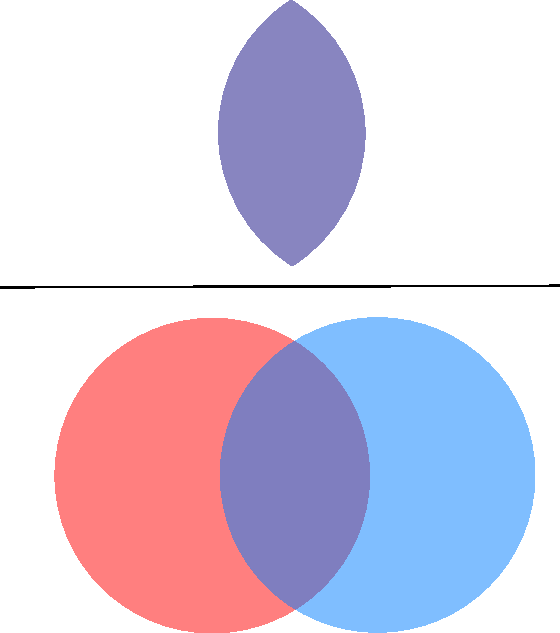
\includegraphics[width=0.5\textwidth]{images/4_jaccard}
		\end{minipage}\hfill
		\pause
		\begin{minipage}[t]{.48\textwidth}
			\centering
			\Large
			Bray-Curtis
			\small
			\medskip
			\begin{equation*}
			BC(A,B) = \frac{2 \times |A \cap B|}{|A| + |B|}
			\end{equation*}
			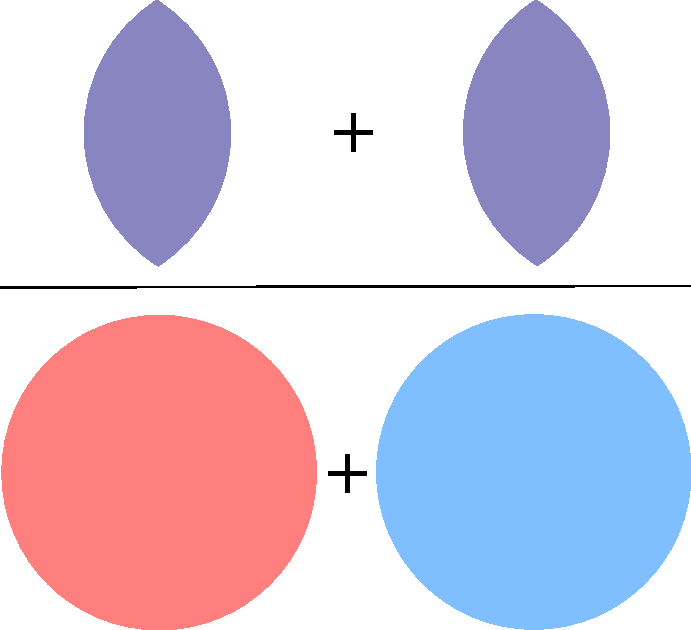
\includegraphics[width=0.6\textwidth]{images/5_bray_curtis}
			
		\end{minipage}\hfill		
	\end{figure}
	\small
	\pause
	
	$J(A,B) = BC(A,B) = 0$ se $A \cap B = \emptyset$\medskip
	
	$J(A,B) = BC(A,B) = 1$ se $A = B$ \phantom{$\cap \emptyset.$}
	
\end{frame}

\begin{frame}
	\frametitle{Reti etichettate e $q$-grammi}
	
	\textit{"Nessun uomo è un'isola, completo in se stesso; ogni uomo è un pezzo del continente, una parte del tutto."}
	\begin{flushright}
		\small \textit{John Donne}
	\end{flushright}
	
	\centering
	\textit{Analizzare non solo l'insieme dei nodi, ma anche la loro interfaccia verso l'esterno!}\\
	
	\pause
	
	Come modellare le interazioni?\\
	
	\pause
	
	\begin{figure}[h]
		\centering
		\begin{minipage}[t]{.49\textwidth}
			\centering
			Rete etichettata\medskip
			
			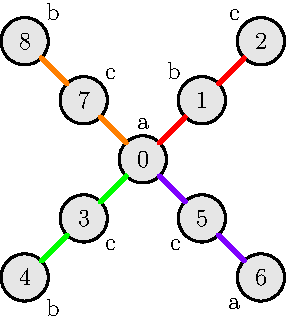
\includegraphics[width=0.5\textwidth]{images/11_labeled}
		\end{minipage}\hfill
		\pause
		\begin{minipage}[t]{.49\textwidth}
			
			\centering
			
			\textbf{q-grammi}: sottosequenza di $q$ elementi consecutivi in un testo
			
			+
			
			\textbf{q-path}: cammino di $q$ nodi \textit{distinti} collegati in un grafo \bigskip
			
			\small\pause
			
			\textbf{Esempio} $3$-grammi che terminano in $0$:
			\begin{itemize}
				\item cba: (\color{red} 2-1-0\color{black})
				\item bca: (\color{green}4-3-0 \color{black}, \color{orange}8-7-0\color{black})
				\item aca: (\color{violet}6-5-0\color{black})
			\end{itemize}
		\end{minipage}
	\end{figure}

	
\end{frame}


\definecolor{RoyalPurple}{rgb}{0.39, 0.19, 0.59}

\begin{frame}
	\frametitle{Frequenze dei $q$-grammi}
	
	\textbf{Notazione:}  
	\small \center	
	$f_X[w] = y \rightarrow$ Il $q$-gramma $w$ ha frequenza $y$ nei $q$-path che terminano in nodi di $X$\medskip
	
	\pause
	
	\textbf{Esempio:}  
	
	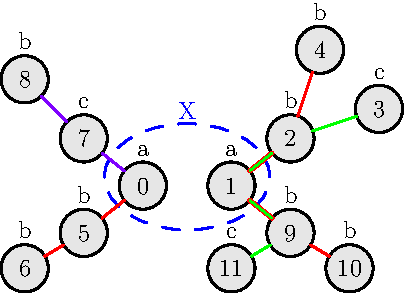
\includegraphics[width=0.4\textwidth]{images/12_freq}
		
	Dato $X = \{0, 1\}$ e $q=3$ abbiamo:
	\centering
	\begin{itemize}
		\item $f_X[bba] = 3$ (path: \color{red}4-2-1\color{black}, \color{red}6-5-0\color{black}, \color{red}10-9-1 \color{black}).
		\item $f_X[bca] = 1$ (path: \color{RoyalPurple}8-7-0 \color{black}).
		\item $f_X[cba] = 2$ (path: \color{green}3-2-1 \color{black}, \color{green}11-9-1 \color{black}).
	\end{itemize}
\end{frame}

\begin{frame}
	\frametitle{Il problema}
	
	\begin{flushleft}
		Dato un grafo $G=(V,E,L)$, etichettato su un alfabeto $\Sigma$, ed un intero $q$,
		calcolare la similarità tra due porzioni di grafo $A, B \subset V$ in base alle frequenze
		dei $q$-grammi dei $q$-path che terminano in nodi di $A$ e $B$.
	\end{flushleft}

	\pause
	\small
	
			
	Estendiamo i due indici ai $q$-grammi, usando $f_A[w]$ e $f_B[w]$ per i $q$-grammi $w$ in $\Sigma^q$:

	\pause 
	\begin{equation*}\label{jaccard-sub}	
		J(A,B) = \frac{|A \cap B|}{|A \cup B|} \implies J(A,B) = \frac{ \Sigma_{w \in \Sigma^{q}} \min(f_{A}[w], f_{B}[w]) }{ \Sigma_{w \in \Sigma^{q}} f_{A \cup B}[w] }
	\end{equation*}

	\begin{equation*}\label{bray-sub}
		BC(A,B) = \frac{2 \times |A \cap B|}{|A| + |B|} \implies BC(A,B) = \frac{ 2 \times \Sigma_{w \in \Sigma^{q}} \min(f_{A}[w], f_{B}[w]) }{ \Sigma_{w \in \Sigma^{q}} (f_{A}[w] + f_{B}[w]) }
	\end{equation*}
	
\end{frame}

\begin{frame}
	\frametitle{Esempio calcolo Bray-Curtis}
	\centering
	\small
	
	Similarità secondo Bray-Curtis tra gli insiemi $A = \{0\}$ e $B = \{1\}$ usando i $3$-grammi 
	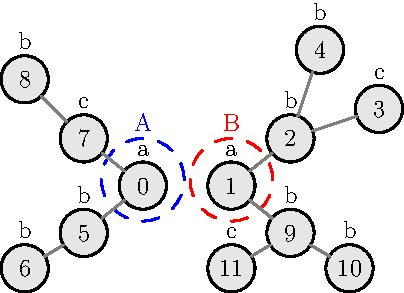
\includegraphics[width=0.4\textwidth]{images/13_bc}
	\begin{table}[h]
	\centering
	\begin{tabular}{|c|c|c|c|c|}
		\hline
		w   & $f_A[w]$ & $f_B[w]$ & $min(f_A[w], f_B[w])$ & $f_A[w] + f_B[x]$ \\ 
		\hline
		bba & 1 & 2 & 1 & 3 \\
		\hline
		bca & 1 & 0 & 0 & 1 \\
		\hline
		cba & 0 & 2 & 0 & 2 \\
		\hline
		\multicolumn{3}{|c|}{Totale} & \color{green}1 &\color{RoyalPurple}6\color{black} \\
		\hline
		%\hline
	\end{tabular}
	\end{table}

	\begin{equation*}
		BC(A,B) = \frac{ 2 \times \Sigma_{w \in \Sigma^{q}} \min(f_{A}[w], f_{B}[w]) }{ \Sigma_{w \in \Sigma^{q}} (f_{A}[w] + f_{B}[w]) } = \frac{2 \times \color{green}1}{\color{RoyalPurple}6\color{black}} = \frac{1}{3}
	\end{equation*}
	
\end{frame}
\begin{frame}
	\frametitle{Applicazioni pratiche}
	
	\pause
	\centering
	\begin{figure}[h]
		\centering
		\begin{minipage}[t]{.49\textwidth}
			\centering
			\textbf{NetInf}\medskip
			
			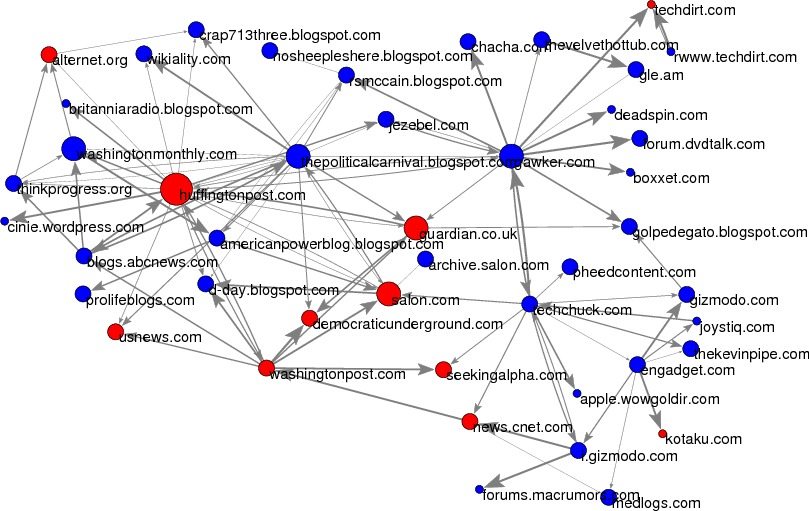
\includegraphics[width=0.9\textwidth]{images/4_netinf}
			\caption{Diffusione delle notizie tra i vari blog e siti di informazione statunitensi\\ \textit{Fonte: SNAP Stanford}}
		\end{minipage}\hfill
		\pause
		\begin{minipage}[t]{.49\textwidth}
			\centering
			\textbf{IMDb}\medskip
			
			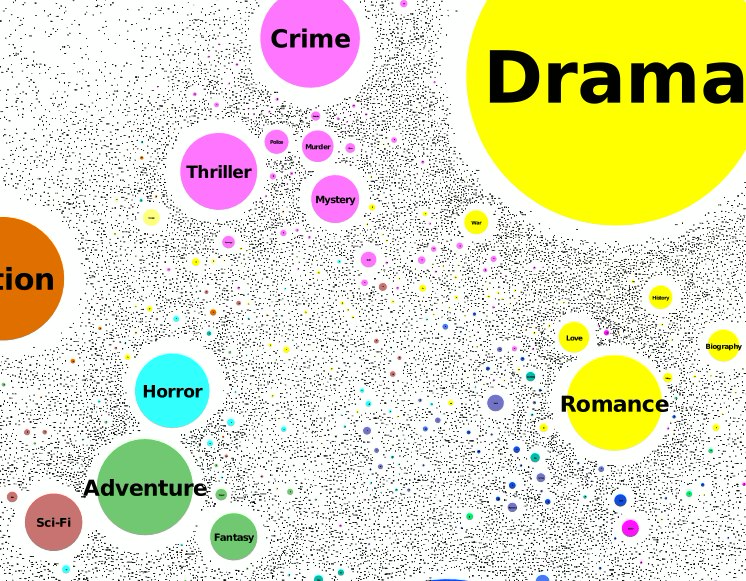
\includegraphics[width=0.9\textwidth]{images/6_imdb}
			\caption{Interazione tra i film con attori in comune\\ \textit{Fonte: IMDb}}
		\end{minipage}
	\end{figure}
\end{frame}

\begin{frame}
	\frametitle{Esempi di similarità}
	
	\pause
	
	\centering
	\begin{table}[h]
		\centering
		\begin{tabular}{c|c|l|l}
			Attore/Attrice & Attore/Attrice  & BC index & J index \\ 
			\hline
			Stan Laurel    & Oliver Hardy    & 0.936167 & 0.774053 \\
			Robert De Niro & Al Pacino       & 0.730935 & 0.231474 \\
			Woody Allen    & Meryl Streep    & 0.556071 & 0.222857 \\
			Meryl Streep   & Roberto Benigni & 0.482909 & 0.160181 \\
			%\hline
		\end{tabular}
		\medskip
		
		$\textsc{IMDb}$, Similarità tra ego-network di attori famosi
	\end{table}
	
	\pause
	
	\begin{table}[h]
		\centering
		\begin{tabular}{c|c|l|l}
			Sito           & Sito            & BC index & J index \\ 
			\hline
			nytimes.com  & huffpost.com       & 0.760524 & 0.388977 \\
			nytimes.com  & washingtonpost.com & 0.732766 & 0.366383 \\
			nytimes.com  & sportingnews.com   & 0.330400 & 0.166200\\
			nytimes.com  & rollingstone.com   & 0.056660 & 0.034336 \\
			%\hline
		\end{tabular}
		\medskip
		
		$\textsc{NetInf}$, Similarità tra siti di informazione
	\end{table}
	
\end{frame}